\section{Punto de Vista de Proyecto}
\subsection{Modelo de Proyecto}
\begin{figure}[h!]
	\centering
	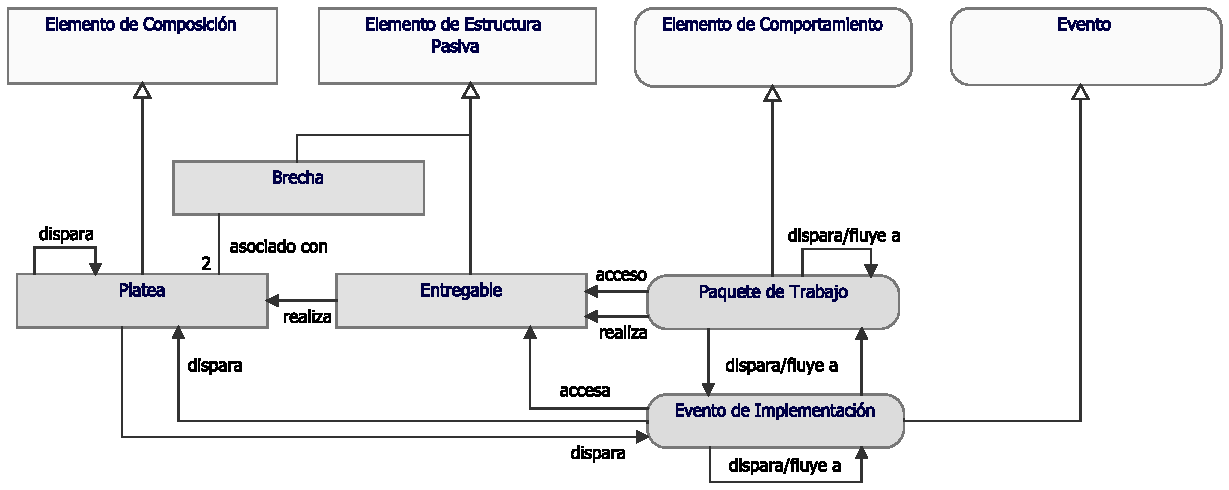
\includegraphics[width=.9\linewidth]{imgs/modelo/Proyecto}
	\caption{Modelo Proyecto}
\end{figure}
El punto de vista del proyecto se utiliza principalmente para modelar la gestión del cambio de arquitectura del proceso de migración desde una situación antigua (estado actual Enterprise
Arquitectura) a una nueva situación deseada (Arquitectura empresarial del estado de destino) tiene

consecuencias sobre la estrategia de crecimiento a medio y largo plazo y la posterior decisión
proceso de fabricación.  Algunas de las cuestiones que deben tener en cuenta los modelos diseñados en
este mirador son:

Desarrollar una Arquitectura Empresarial completa para toda la organización es una tarea que puede
 requieren varios años.

Todos los sistemas y servicios deben permanecer operativos independientemente del presunto modificaciones y cambios de la Arquitectura Empresarial durante el proceso de cambio.

El proceso de cambio puede tener que lidiar con estándares tecnológicos inmaduros (por ejemplo,
mensajería, seguridad, datos, etc.).

El cambio tiene graves consecuencias para el personal, la cultura, la forma de trabajar y
organización. Además, hay varios otros aspectos de gobernanza que podrían limitar la transformación del proceso, como cooperación interna y externa, gestión de cartera de proyectos, gestión de proyectos (entregables, metas, etc.), planificación de meseta, aspectos financieros y legales, etc.

\subsection{Caso  de Proyecto}
\begin{figure}[h!]
	\centering
	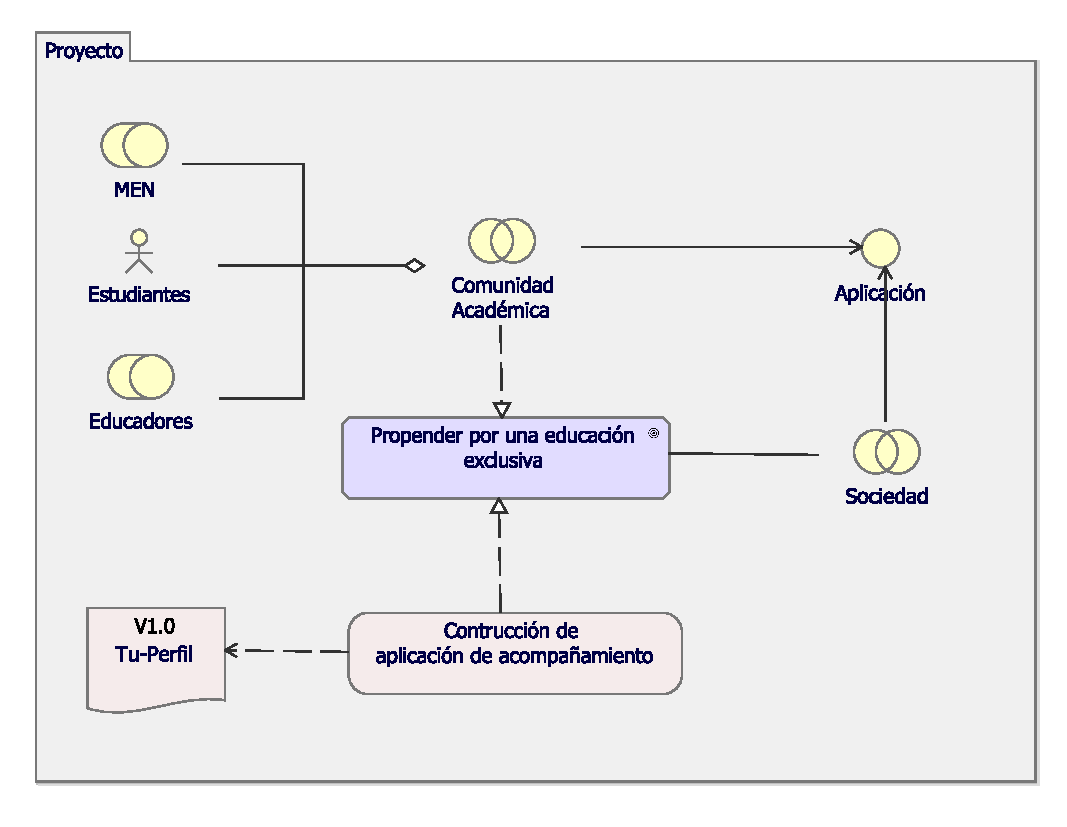
\includegraphics[width=.9\linewidth]{imgs/caso/proyecto/proyecto.pdf}
	\caption{Caso Proyecto}
\end{figure}
El objetivo que se propone por parte de la organización planteado en la capa motivacional "propender por una educación exclusiva" del cual se extiende o afecta a la comunidad académica que se compone Pone a su vez del MEN, de los estudiantes y de los educadores. Para dar alcance a este objetivo se pretende realizar la construcción de una aplicación de acompañamiento profesional, que permite el despliegue de Tu-Perfil en su versión 1.0.